\subsubsection{Introducción}

Tras el desarrollo de robots primigenios con funcionalidades concretas se planteó la posibilidad de integrar movimiento por el terreno en los mismos para poder realizar nuevas tareas u otras de forma más eficiente. En este ámbito se invirtió para lograr avances en esquivar objetos del escenario o en sistemas para andar basados en animales cuadrúpedos o bípedos como nosotros. A continuación analizamos de forma cronológica estos hechos.

\subsubsection{RB5X de RB Robot Corporation}
Un inicio en la movilidad en los robots fue incorporarles ruedas u orugas como herramientas para su desplazamiento por el suelo. Estos tipos de movimientos eran básicos, tales como ir hacia delante, hacia atrás o hacia los lados. Un avance en el movimiento inteligente lo protagonizó el Stanford's Cart, el cual fue programado con sensores para desplazarse de una punta a otra de un recinto esquivando los objetos a su paso. Este movimiento inteligente era realizado gracias a un sistema de Visión por Computador que incluía el mismo. Tras esto surgieron nuevos intentos como el RB5X, un robot de pequeñas dimensiones capaz de desplazarse y evitar obstáculos o, en caso de no poder evitarlos, capaz de reconstruir su trayectoria tras impactar con algún objeto.

\vspace{10px}

El robot se ideó de forma multipropósito, puesto que los módulos que integraba eran programables por lo que las empresas tomaron el diseño y lo adecuaron a las tareas que se querían. El robot tuvo variantes tales como asistentes personales a los cuales les podías dar órdenes como recoger el periódico y a través de un brazo robótico que incluía poder interactuar con el medio. Además se le desarrolló una interfaz oral básica para poder darles órdenes mediante la voz. Además era capaz de aprender de su entorno.

\subsubsection{Phony Pony}

Tras los intentos de hacer robots que incorporasen ruedas u orugas la Universidad de California del Sur realizó el desarrollo del que se conoce como primer robot cuadrúpedo llamado Phony Pony. El diseño de este robot se realizó en 1968 (anterior a RB5X) por los profesores e investigadores Frank y McGhee.

\vspace{10px}

El robot intentaba imitar las articulaciones de los animales cuadrúpedos que conocemos de forma que lo desarrollaron con dos articulaciones: la cadera y la rodilla. De esta forma el robot podía mover la pierna hacia delante y además flexionarla. La velocidad del movimiento de las patas era extremadamente lenta, ya que al igual que ocurría con el Stanford Arm (contemporáneo a Phony Pony) los elementos eléctricos empleados en el movimiento estaban muy limitados. El Phony Pony era capaz de imitar comportamientos tales como andar, arrastrarse, agacharse o trotar.

\vspace{10px}

El control de este robot se realizaba de forma remota gracias a la tecnología desarrollada ya en esa época. Internamente el robot estaba diseñado mediante patrones de movimiento, de forma que estaba implementado con un autómata finito que tomaba las transiciones del mismo tras recibir la entrada del mando de control.

\subsubsection{WAP1}
En primer paso que se dio entorno a la idea de realizar un robot bípedo tuvo lugar en 1969 en la Universidad de Waseda en Japón. El robot WAP1 (Waseda's antropomorphic pneumatically-activated pedipulators) fue diseñado por el doctor Ichiro Kato.

\vspace{10px}

El doctor Ichiro Kato trabajaba por aquel momento en el terreno médico y empezó a intentar desarrollar músculos artificiales para poder sustituir músculos defectuosos en sus pacientes. El estudio desarrolló una serie de dispositivos que al hincharse adquirían las formas que ellos necesitaban para simular el comportamiento de un músculo. Estas investigaciones darían sus frutos plasmándose en el primer robot bípedo creado. Los músculos que permitían el movimiento de WAP1 estaban hechos de goma y se inflaban con actuadores neumáticos. Este primer robot no era capaz más que de andar muy lentamente controlando el flujo de aire que se llevaba hacia las piezas de goma. Estas técnicas hacían que WAP llegara a tardar mucho tiempo en completar un paso, además de que no estaba pensado para andar una distancia dando pasos de forma consecutiva.

\vspace{10px}

En los dos siguientes años el doctor Ichiro Kato mejoró el diseño del WAP1 creado el WAP2 y el WAP3. La segunda versión de estos robots tuvo una mejora en la fuerza que los músculos eran capaces de aplicar sobre la estructura del mismo, pudiendo ahora levantar más peso y tener una estructura más robusta. La última versión fue desarrollada en 1971 y en esta el robot ya era capaz de rotar su movimiento, por lo que ya no tenían que ser movimientos rectos y, además, era capaz de superar pequeños obstáculos tales como ligeras inclinaciones o incluso escaleras de pequeño tamaño. Para poder desarrollar todo esto no sólo fueron necesarios los músculos artificiales del doctor Kato, si no además sus estudios en el control y mejora de la postura con lo que fueron capaces de controlar el centro de gravedad del robot, cosa completamente imprescindible para caminar sobre dos piernas.

\subsubsection{WL-9DR}
Tras los avances del doctor Ichiro Kato se intentó agilizar el movimiento de estos robots, puesto que el tiempo que había que esperar hasta que el WAP era capaz de avanzar un paso hacía que no fuera práctico su uso, ya que los robots que empleaban ruedas por ejemplo eran mucho más ágiles. Entre los años 1979 y 1980 la Universidad de Waseda desarrolló el WL-9DR bajo la dirección del doctor Kato, al igual que con sus predecesores los WAP.

\vspace{10px}

El funcionamiento de esta máquina era mediante actuadores hidráulicos que operaban más rápidamente que los diseñados para WAP. Así mismo el control de este robot se hacía mediante un procesador de 16 bit conectado al robot mediante cables. El WL-9RD era capaz de dar un paso en 10 segundos, además de realizar ciclos completos andando, es decir, encadenar pasos para avanzar desde el punto de partida a un punto meta que se le fijaba. La velocidad con la que avanzaba era tan lenta que sus creadores no podían podían denominar al robot como dinámico, por lo que se le conoce como el primer robot bípedo cuasi-dinámico.

\vspace{10px}

El robot tenía un sistema de pesos que mantenía el equilibrio del mismo como se requiriera, por ejemplo si el robot estaba estático se centraba el punto de apoyo y se mantenía la postura tanto por la gran base rectangular de sus pies como por los pesos centrados. Si se quería dar un paso hacia delante el robot alzaba alguna de las piernas y se cambiaba el centro de los pesos un poco hacia delante, de forma que el robot se inclinara ligeramente para seguir con el siguiente paso. Para poder andar solamente 0.5 metros el robot requería sobre una docena de pasos llevándole entorno a un minuto completar dicha distancia.

\subsubsection{Aquarobot}
Tras los robots anteriormente mencionados (que sentaron precedentes en el tema de caminar) se siguieron desarrollando las técnicas que se empleaban en el equilibrio y las partes móviles de los mismos tal y como veremos en las siguientes secciones. Entre estos robots surgieron algunos proyectos que intentaron ir un poco más allá como el Aquarobot cuyo objetivo era ser capaz de andar bajo el agua.

\vspace{10px}

En el instituto de investigaciones de puertos de Japón se pensó en que sería útil que los operarios que tenían que trabajar bajo el agua dispusieran de facilidades para hacer la tarea más rápida y sencilla. Uno de los trabajos que más tiempo llevaban en el puerto eran los de inspección bajo el agua para certificar el estado de las estructuras o diagnosticar algún tipo de fallo que se debía solventar. Por ello en el año 1984 se desarrolló la primera versión del Aquarobot, llegando a tener este hasta tres versiones diferentes haciendo mejoras sobre lo ya propuesto.

\vspace{10px}

El diseño básico del robot era una estructura con 6 patas capaz de andar bajo el agua. Los motores que empleaban eran de corriente continua (no neumáticos) colocados en cada una de las patas que iban selladas de forma estanca para impedir la entrada del agua. Además el robot era controlado por un pequeño procesador incluido en el mismo al que se le conectaban cables para comunicarlo con una computadora o un mando de control. El Aquarobot disponía asimismo de una cámara integrada que permitía ver en tiempo real lo que el robot observaba, de forma que los técnicos podían visualizar el estado del puerto sin necesidad de bajar ellos al agua.

\vspace{10px}

Cada pata tenía 3 grados de libertad con los que el robot podía andar y rotar sobre sí mismo. El peso aproximado de este robot era de unos 857 kilogramos en su primera versión y de unos 280 en la tercera. El sistema con el que se manipulaba al robot y los patrones de movimiento que se le definían en su propio procesador estaba programados en C++. El tiempo en el que el robot era capaz de responder a las órdenes que se le daban era de unos 50 milisegundos, gracias a la conexión que se tenía mediante cable.

\subsubsection{Honda y el gran avance}
La compañía Honda Motors, normalmente conocida por la fabricación de coches, tuvo un papel muy importante en el desarrollo de los robots antropomórficos y bípedos con sus series de robots, desde la serie E experimental, pasando por la P hasta los más que conocidos robots ASIMO que perduran actualmente.

\vspace{10px}

La serie de robots Honda E contó con 7 modelos, desde el 0 hasta el 6 desarrollados entre los años 1986 y 1993. Esta serie experimental comenzó en el mismo punto que el robot WAP, desarrollando un sistema que podía caminar sobre dos piernas. Estos robots, desde la versión 0, mejoraron enormemente los tiempos conseguidos por sus predecesores necesitando, ``únicamente'', 5 segundos para dar un paso completo. Este modelo contaba con 6 grados de libertad y con las articulaciones similares a las de una pierna humana, una cadera, la rodilla y el tobillo. En la versión 1 se mejoró la velocidad de movimiento pero se aumentó el peso haciendo que fuera notablemente más grande que su versión anterior, además se le añadió un sistema mucho más complejo de articulaciones que le permitían tener 12 grados de libertad. En las versiones 2,3,4 y 5 se mejoró tanto el peso como la velocidad al andar, logrando que el robot anduviera de forma autónoma y dinámica llegando a los 4.7 kilómetros por hora. Cabe destacar que el diseño acabó con una cabeza muy grande y un peso de 150 kilogramos (comparados con los 16.5 de la versión 0). En la última versión no se modificó tanto el diseño y la velocidad al andar, si no que se centraron en que el robot fuera capaz de controlar el equilibrio de forma inteligente y fuese capaz de esquivar obstáculos e incluso no andar sobre un suelo liso.

\vspace{10px}

Tras el gran avance que lograron los ingenieros de Honda en cuanto a la capacidad de desplazamientos de la serie E, decidieron tomar todos esos avances y añadir más elementos para que pareciera cada vez más una persona. Tras la serie E vino la P con la intención de tomar lo obtenido de forma experimental en la anterior serie para continuar su camino hacia los robots antropomórficos. Estos robots fueron desarrollados entre los años 1993 y 2000. El primer modelo de la serie P supuso una transición en la cual se le añadieron brazos que, aunque no eran capaces de llevar una carga, le servían al robot para interactuar con el medio con acciones tales como abrir puertas o encender y apagar interruptores. En el modelo P2 Honda quiso marcar un precedente en la historia de la robótica haciendo que se pudiera desplazar andando, subir escaleras, empujar objetos e incluso llevar carga en las manos. El robot fue el primero en el que no se utilizaron cables para la comunicación con el mismo, para lo cual llevaba una batería incluida que permitía que trabajase alrededor de unos 15 minutos. La opinión pública se sorprendió enormemente, ya que este fue el primer robot conocido que tuvo un movimiento muy similar al humano. Tras el segundo modelo Honda sacó el P3, cuyo objetivo con respecto a la versión anterior era reducir el peso, cosa que consiguieron ya que se pasó de 210 kilogramos a 130 sin variar las dimensiones del mismo más que en la profundidad del cuerpo del robot. El diseño además adquirió una semejanza mayor aún a los humanos con respecto al P2 y se mejoró la eficiencia de uso en la batería lo que permitió una autonomía de 25 minutos en lugar de los 15 minutos del P2. Por último se sacó el Honda P4, el que fue el último en la serie P de robots. Las dimensiones no variaron con respecto al P3 pero si el peso que se redujo a 80 kilogramos. Además este robot fue el que consiguió un movimiento más completo de la serie P con 34 grados de libertad contando brazos y piernas pero no se profundizó especialmente en esta versión puesto que los robots ASIMO estaban ya en desarrollo y Honda decidió acabar esta serie para dedicar todos sus esfuerzos en la nueva gama de robots.

\vspace{10px}

La serie de robots ASIMO o (Advanced Step in Innovative Mobility) fueron la continuación de la serie P de Honda en cuanto a la creación de un robot humanoide. Los robots ASIMO tuvieron diferentes revisiones, esta vez no divididas en diferentes modelos. La primera versión se sacó a la luz en el año 2000 para después tener nuevas mejoras en los años 2002, 2005, 2007 y 2011. Los ASIMO comenzaron teniendo una altura de 120 centímetros y 54 kilogramos de peso, un gran avance comparando los pesos y alturas con los obtenidos en la serie P que llegaban a pesar 210 kilogramos. ASIMO mejoró en la velocidad en la que andaba pasando de 1.6 kilómetros por hora a 2.7 kilómetros por hora. En sus primeros modelos ASIMO no era capaz de correr pero en el modelo de 2004 la funcionalidad se añadió comenzando a correr a 3 kilómetros por hora hasta los 9 de la versión de 2011. La batería que incorporaban los Honda P fue reutilizada en las primeras versiones de los ASIMO pero ésta cambió a una batería de ion de litio desde el 2004 para llegar a dar una hora completa de batería en uso mixto (andando y corriendo). Además los grados de libertad que obtuvo la versión de 2011 fueron 57, un número muy superior a los 26 del modelo del año 2000 que permitía movimientos no sólo de brazos y piernas si no también movimientos completos de los dedos de la mano con lo que la última versión es capaz de hacer gestos con la misma y movimientos complejos parecidos a los que podemos realizar con nuestra mano. Además en la última versión se le añadió un sistema de voz con el que las personas nos podemos comunicar con ASIMO para pedirle tareas específicas. En su última versión el robot ASIMO es capaz de reconocer el entorno que le rodea mediante cámaras y sensores de visión incorporados en su casco con los cuales ASIMO no sólo es capaz de interactuar con las personas por voz, si no que también es capaz de analizar los movimientos y comportamientos de las mismas para actuar en función de ello. Además en cuanto a la interfaz oral no sólo responde mediante altavoces para continuar la conversación, si no que además también gesticula para dar una interacción más humana.

\begin{figure}[!h]
	\centering
	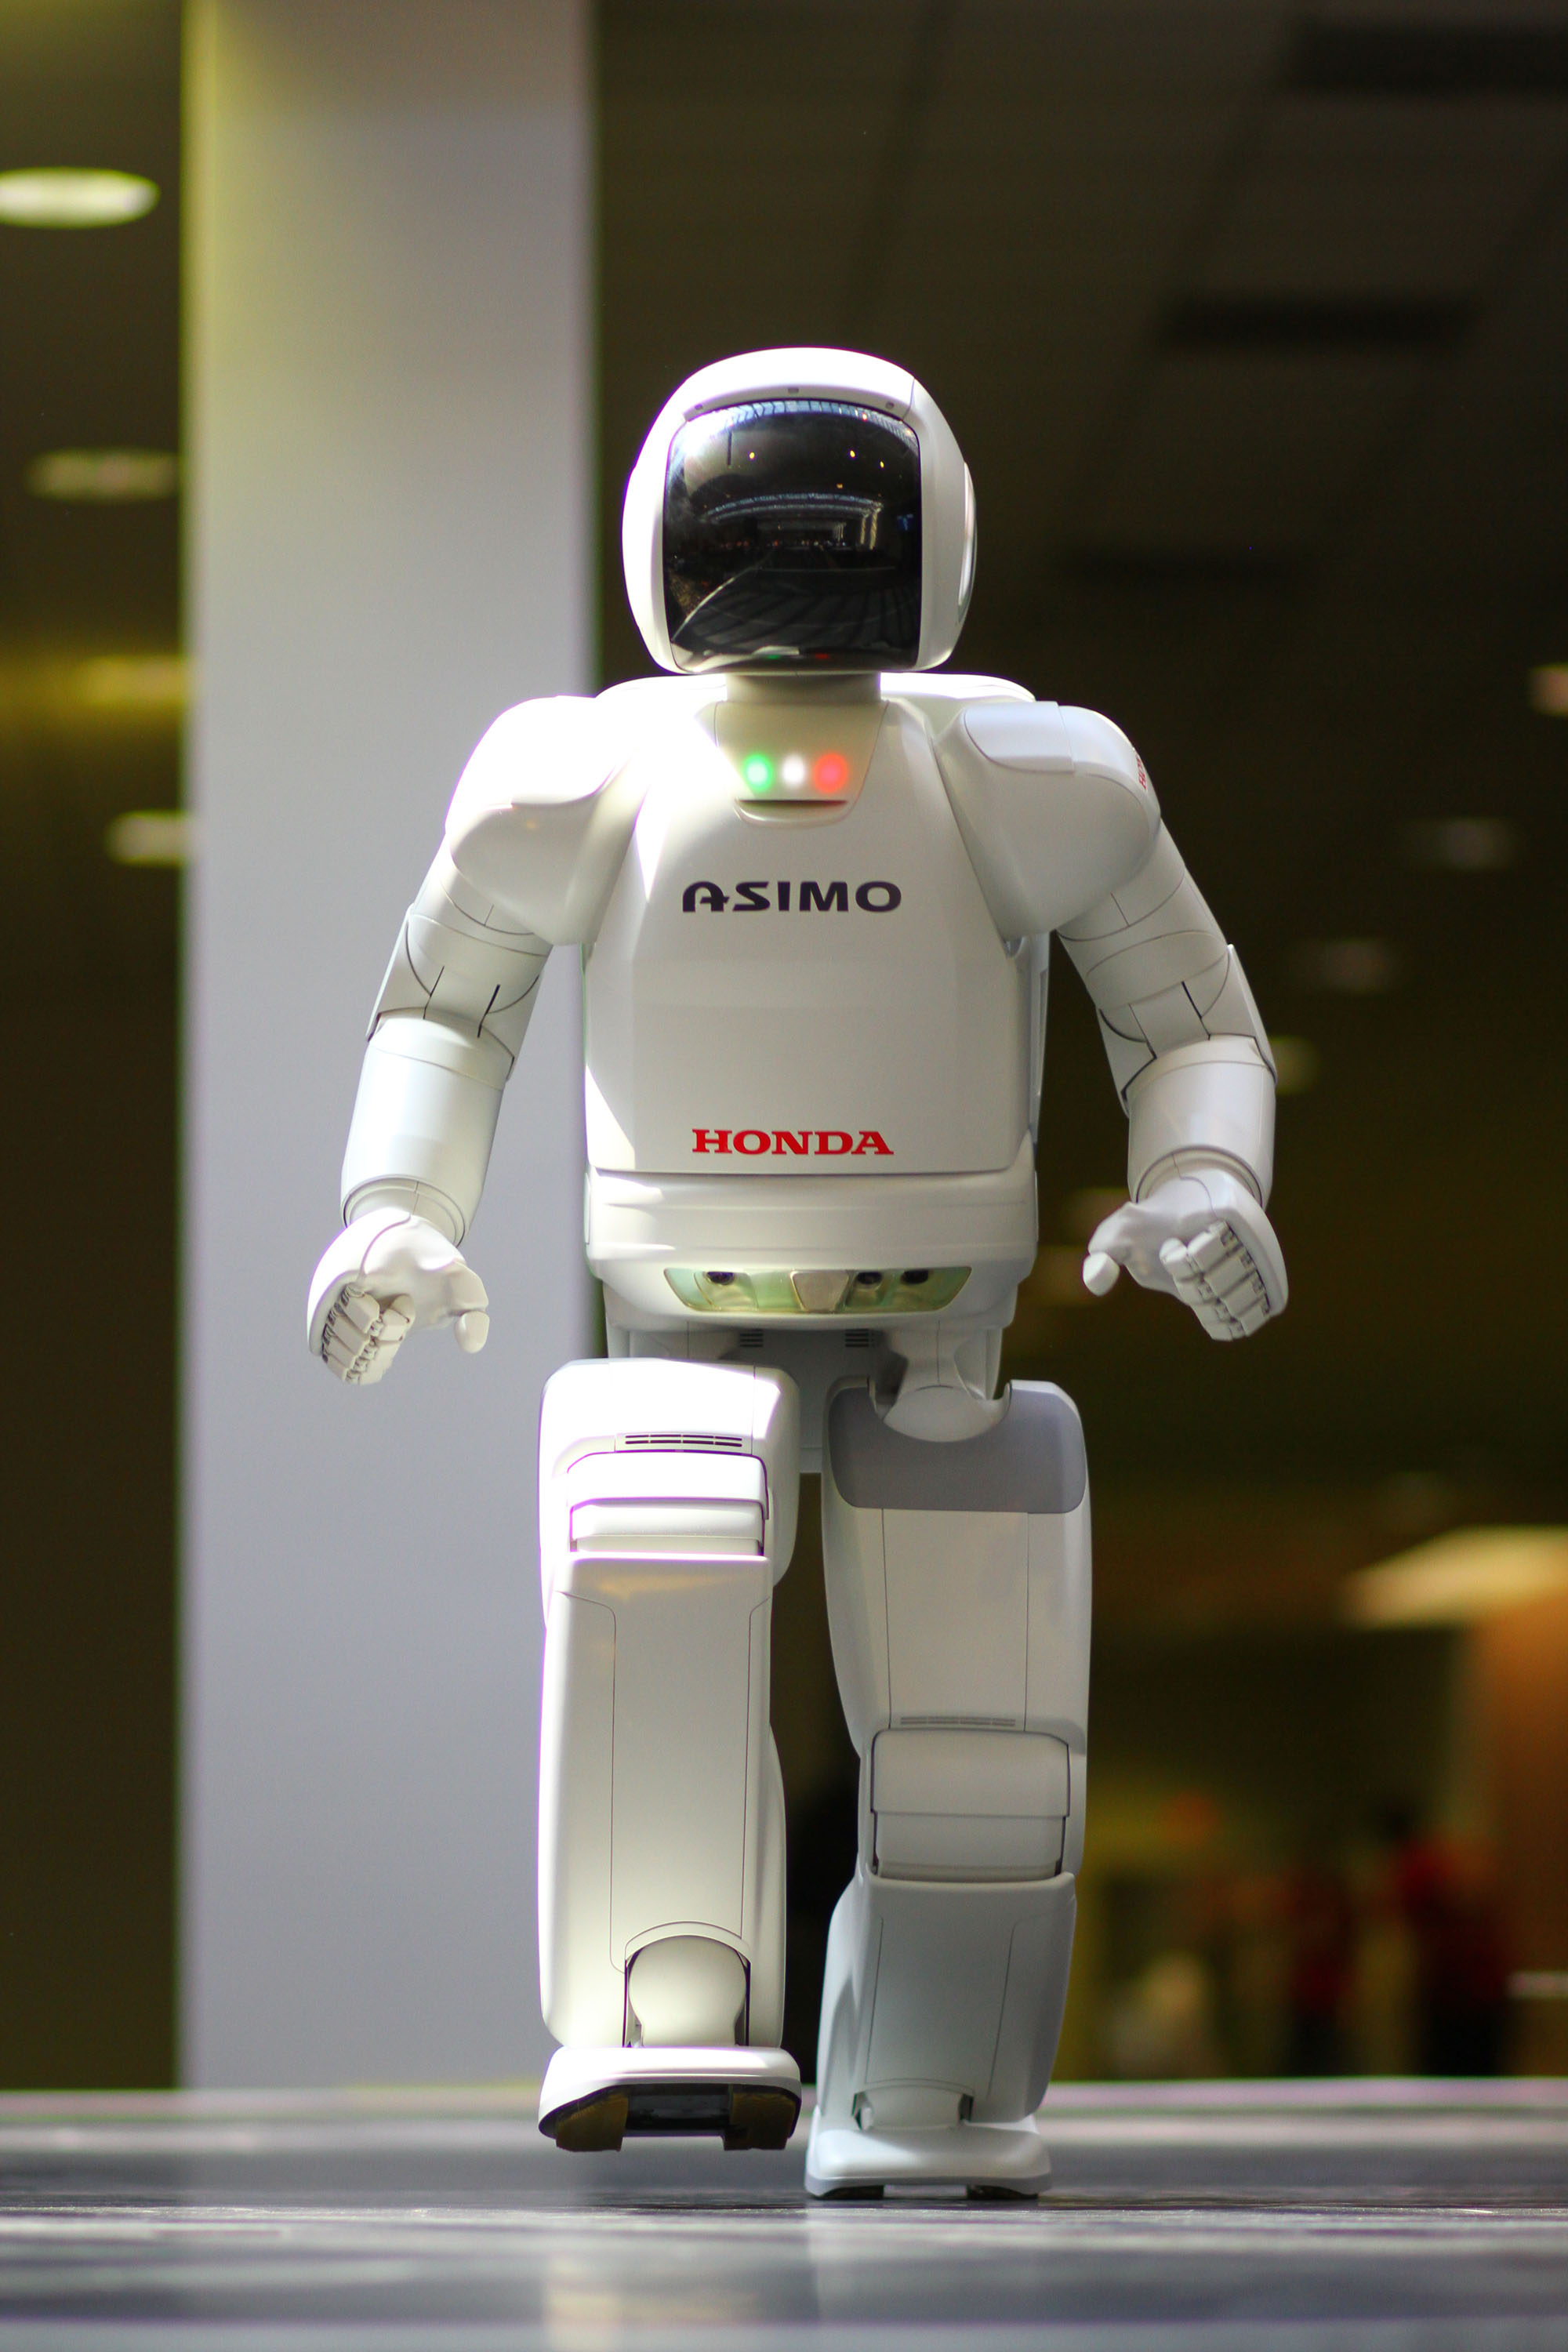
\includegraphics[scale=0.2]{./EtapaModerna/Imagenes/asimo.jpg}
	\caption{ASIMO (\href{https://es.m.wikipedia.org/wiki/Archivo:ASIMO_4.28.11.jpg}{Wikimedia})}
	\label{fig:asimo}
\end{figure}

Con los robots ASIMO Honda completó una era en cuanto a los movimientos en la robótica, al conseguir un movimiento al caminar natural y rápido y una interacción con el medio a través de las manos y brazos muy extensa. Tras esto los robots antropomórficos han seguido avanzando pero todos utilizando en gran medida la senda que Honda marcó con su series E, P y ASIMO.
